\begin{figure}[ht!]
    \begin{subfigure}{.5\textwidth}
    \centering
    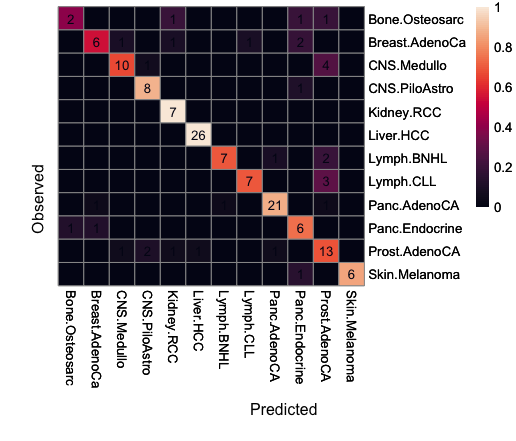
\includegraphics[width=\textwidth,height=0.9\textwidth]{graphics/confusion_matrix_2-submotifs.png}
    \caption{2-submotifs}
    \label{fig:confusion_2-submotifs}
    \end{subfigure}
    ~
    \begin{subfigure}{.5\textwidth}
    \centering
    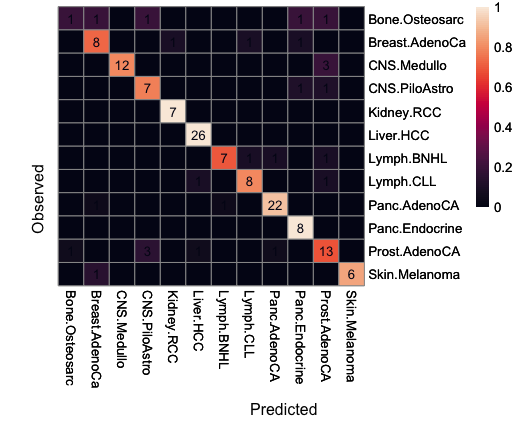
\includegraphics[width=\textwidth,height=0.9\textwidth]{graphics/confusion_matrix_3-submotif.png}
    \caption{3-submotifs}
    \label{fig:confusion_3-submotifs}
    \end{subfigure} \\
    
    \caption{\textbf{Representative confusion matrix, coloured by the percentage of predicted values over row total, for (a) 2-submotifs, (b) 3-submotifs.} This is an extension of Figure \ref{fig:f1_sce_submotif}.}
    \label{fig:apdx_ml_submotifs}
\end{figure}